
% --------------------------------------------------------------------------------------------------
% Kommando Beispiele
% --------------------------------------------------------------------------------------------------

% Referenz auf z.B. Kapitel
\chapter{Related Work}
\label{c:related_work}

There are two types of related work for this BA thesis. The first consists of already existing OWASP MASTG reference apps for android. The second is about academic works making use of the MASTG, an industry standard, and its reference apps. 



% Struktur
\section{State-Of-The-Art in OWASP MASTG Reference Apps}
At the time of writing, there are currently 19 MASTG reference apps listed on the OWASP page. To evaluate the state of the art of these apps, it is necessary to examine each one of them in order to identify and categorize their implemented weaknesses. Only 8 of said apps had both available sourcecode as well as some form of documentation of their weaknesses. These were then mapped by the author to their corresponding OWASP MASWE counterparts.


\subsection{Findings}
Across the 8 evaluated OWASP MASTG reference apps, 162 weaknesses where mapped to their respective MASWE counterpart and grouped by their vulnerability category (Storage, Crypto, Auth, etc.).

\subsubsection{Lack of vulnerability documentation}
A reoccurring issue with many of the reference apps is their documentation of the implemented vulnerabilities. Multiple of the reference apps do not have any documentation of their weaknesses at all, which led to their exclusion from this evaluation. Those apps that do have some form of documentation are often incomplete, and almost always only consist of a single list, naming the implemented weaknesses and leaving it at that. None of the apps map the implemented weaknesses to their OWASP MASWE counterparts, despite them being a MASTG reference app, designed for this very purpose. Only one app \todo{add source and specific names of mentioned apps here, just in general less vague than is now.} actually documents what the weaknesses entail, how they are implemented, and how to fix or exploit them. 

Since these apps are meant by OWASP to be educational, it does not suffice to only implement the weaknesses and leave as is. The app developed in this BA thesis aims to fill this hole by not only documenting all implemented weaknesses, but adding documentation for each specific weakness, consisting of where it is found, what lines of code are of relevancy, how to exploit them, aswell as how to fix them.

\subsubsection{Uneven distribution of vulnerability coverage}
At the time of writing, there are a total of 117 MASWE vulnerabilities across 8 categories documented by OWASP. Of these 117 vulnerabilities, only 38 are actually covered by any of these reference apps. 


\todo{CREATE GRAPH DISPLAYING VULNERABILITY COVERAGE GROUPED BY APP, INSERT HERE}
Since there are 162 weaknesses implemented, but only 38 different types of weaknesses as used by the MASTG, this leaves a total of 79 vulnerabilities, as documented and classified by OWASP MASWE and referenced in the MASTG, completely without representation. This further means that there are some vulnerabilities which are heavily favoured to be implemented in these reference apps, with them being added in high frequency, while many more vulnerabilities see no coverage at all.

To make this point more clear; the ten most frequently covered vulnerabilities are in total implemented 75 times, meaning that they represent 46\% (75/162) of all implemented vulnerabilities, despite only covering 8.5\% (10/117) vulnerabilities as referenced by MASTG. The most frequently implemented vulnerability, as seen in Figure 1, is MASWE-0066, which deals with insecure intents. Of the ten most frequently covered vulnerabilities, 5 are of the category "Platform".

\begin{figure}[htbp]
  \centering
  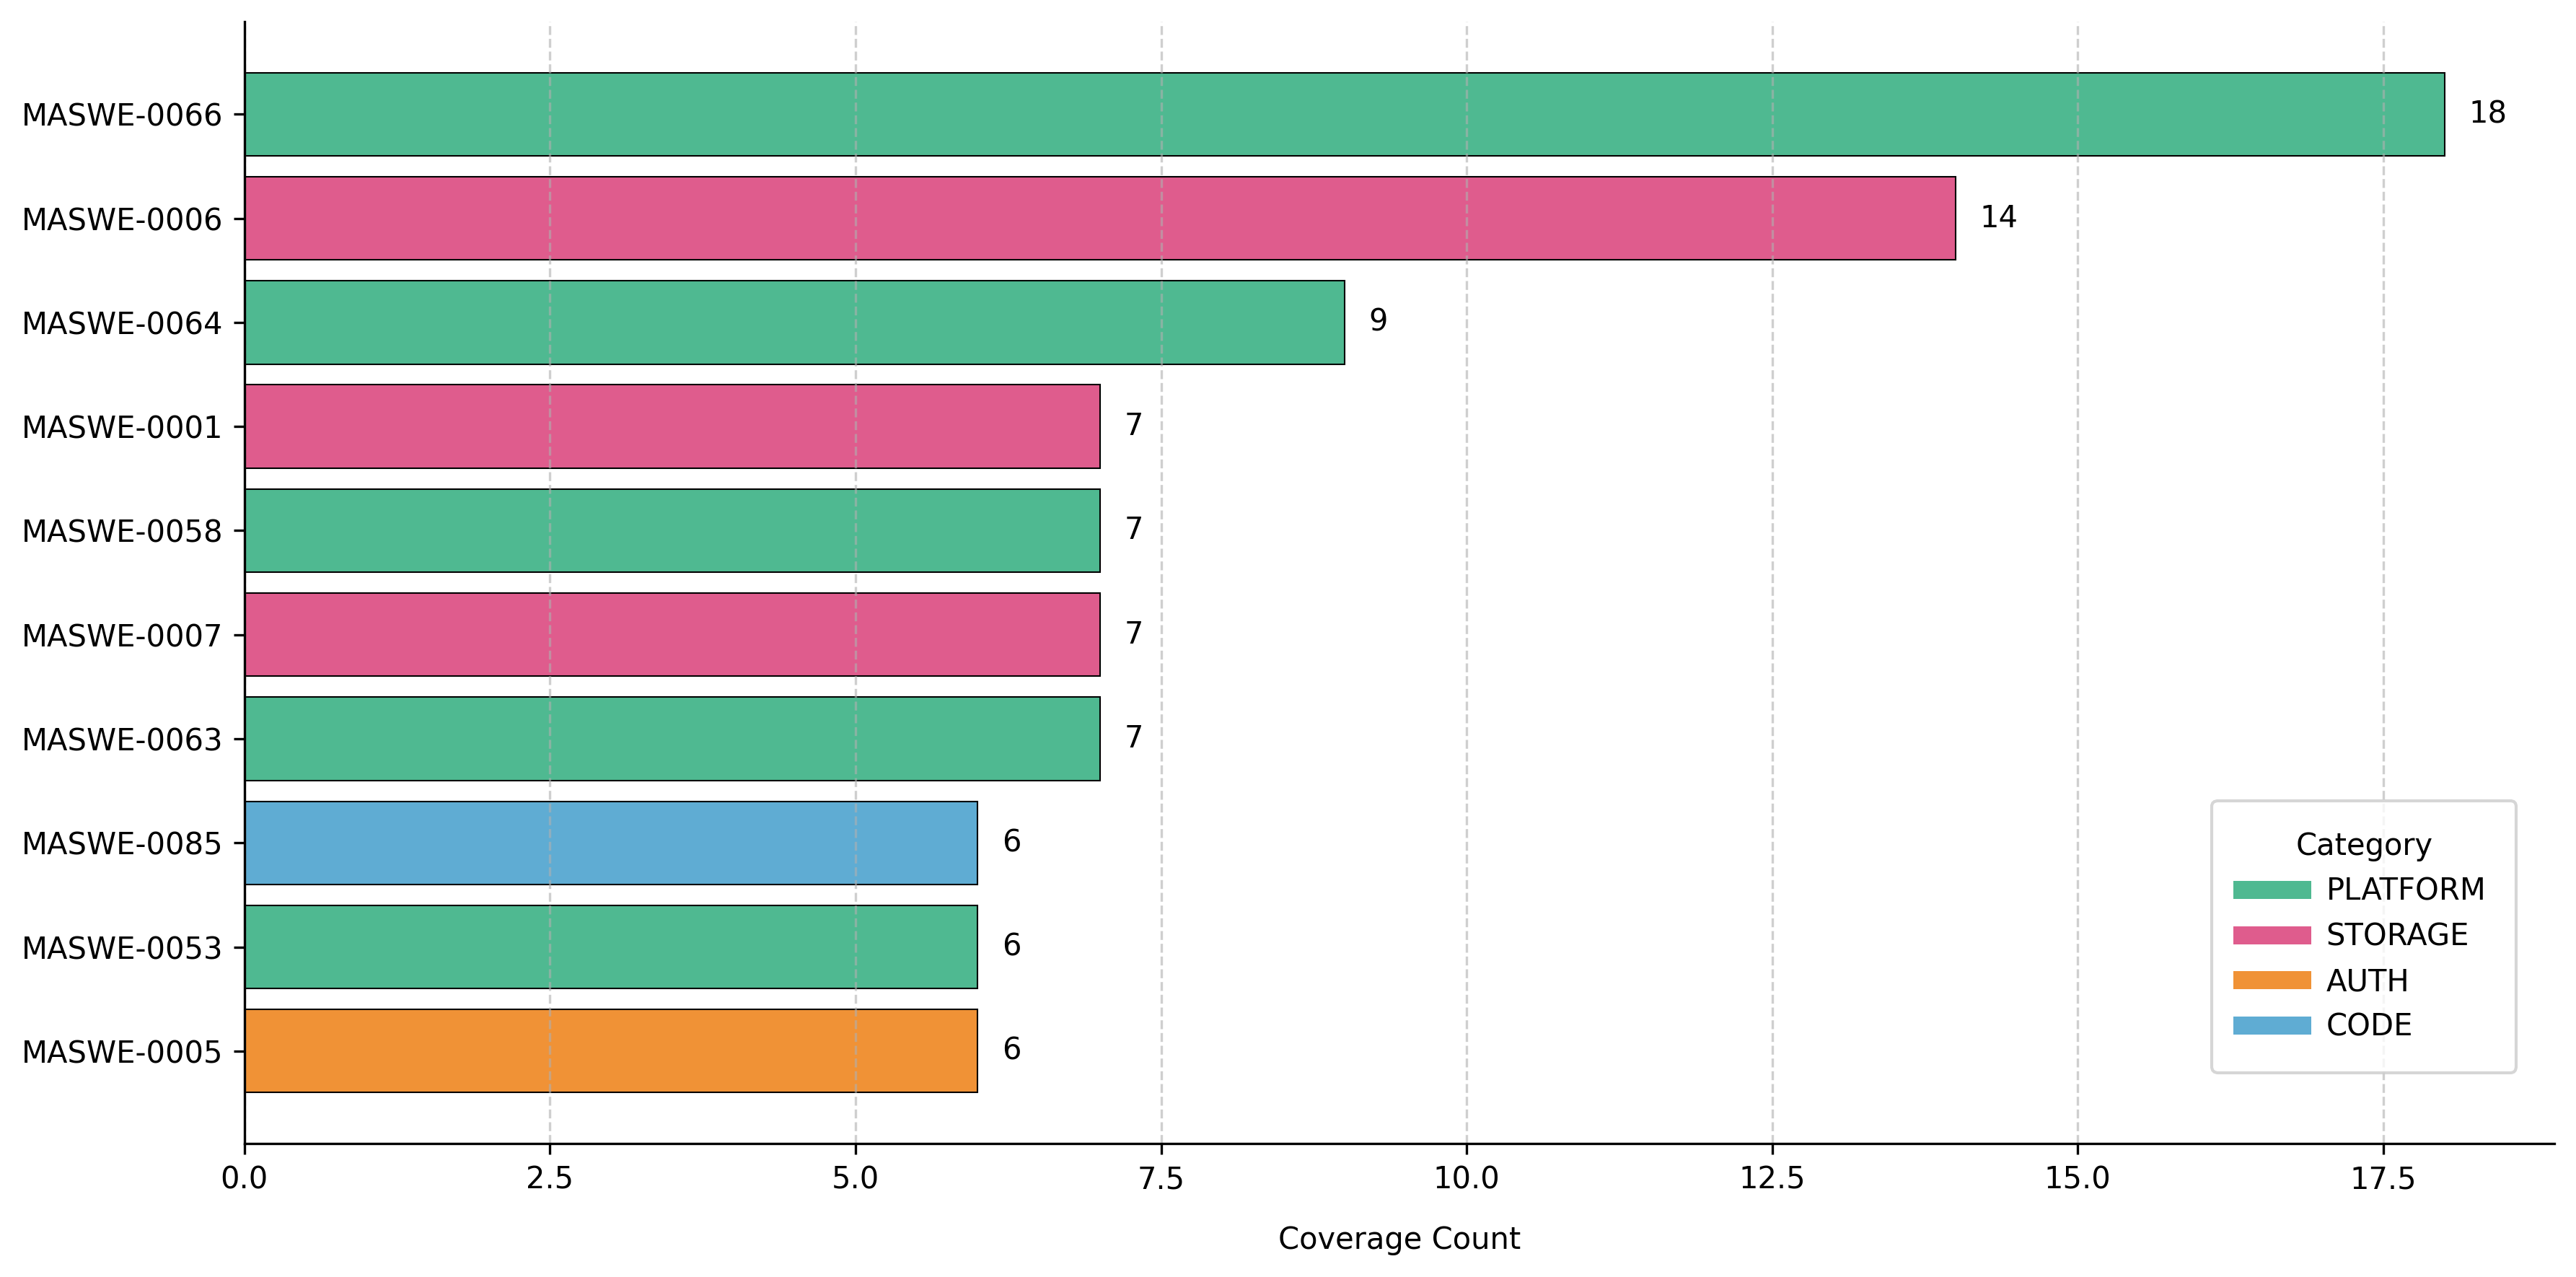
\includegraphics[width=1.0\textwidth]{figures/related_work/top_10_vulnerabilities.png}
  \caption{Barplot depicting the ten most frequently covered types of OWASP MASWE vulnerabilities, colored according to their respective category.}
  \label{fig:model}
\end{figure}

\subsubsection{Coverage of vulnerability categories}
There is not only a favouring of certain specific MASWE vulnerabilities, but also an uneven coverage of the vulnerability categories themselves as well. When viewed percentage-wise, as seen in figure 2.2., some categories see a high percentage of their vulnerabilities covered, such as Platform with 72.7\% or Storage with 66.7\%, while others see very little to no coverage at all, such as both Crypto and Auth with only 10\% and worst of all Privacy with a vulnerability coverage of 0\%.

\begin{figure}[htbp]
  \centering
  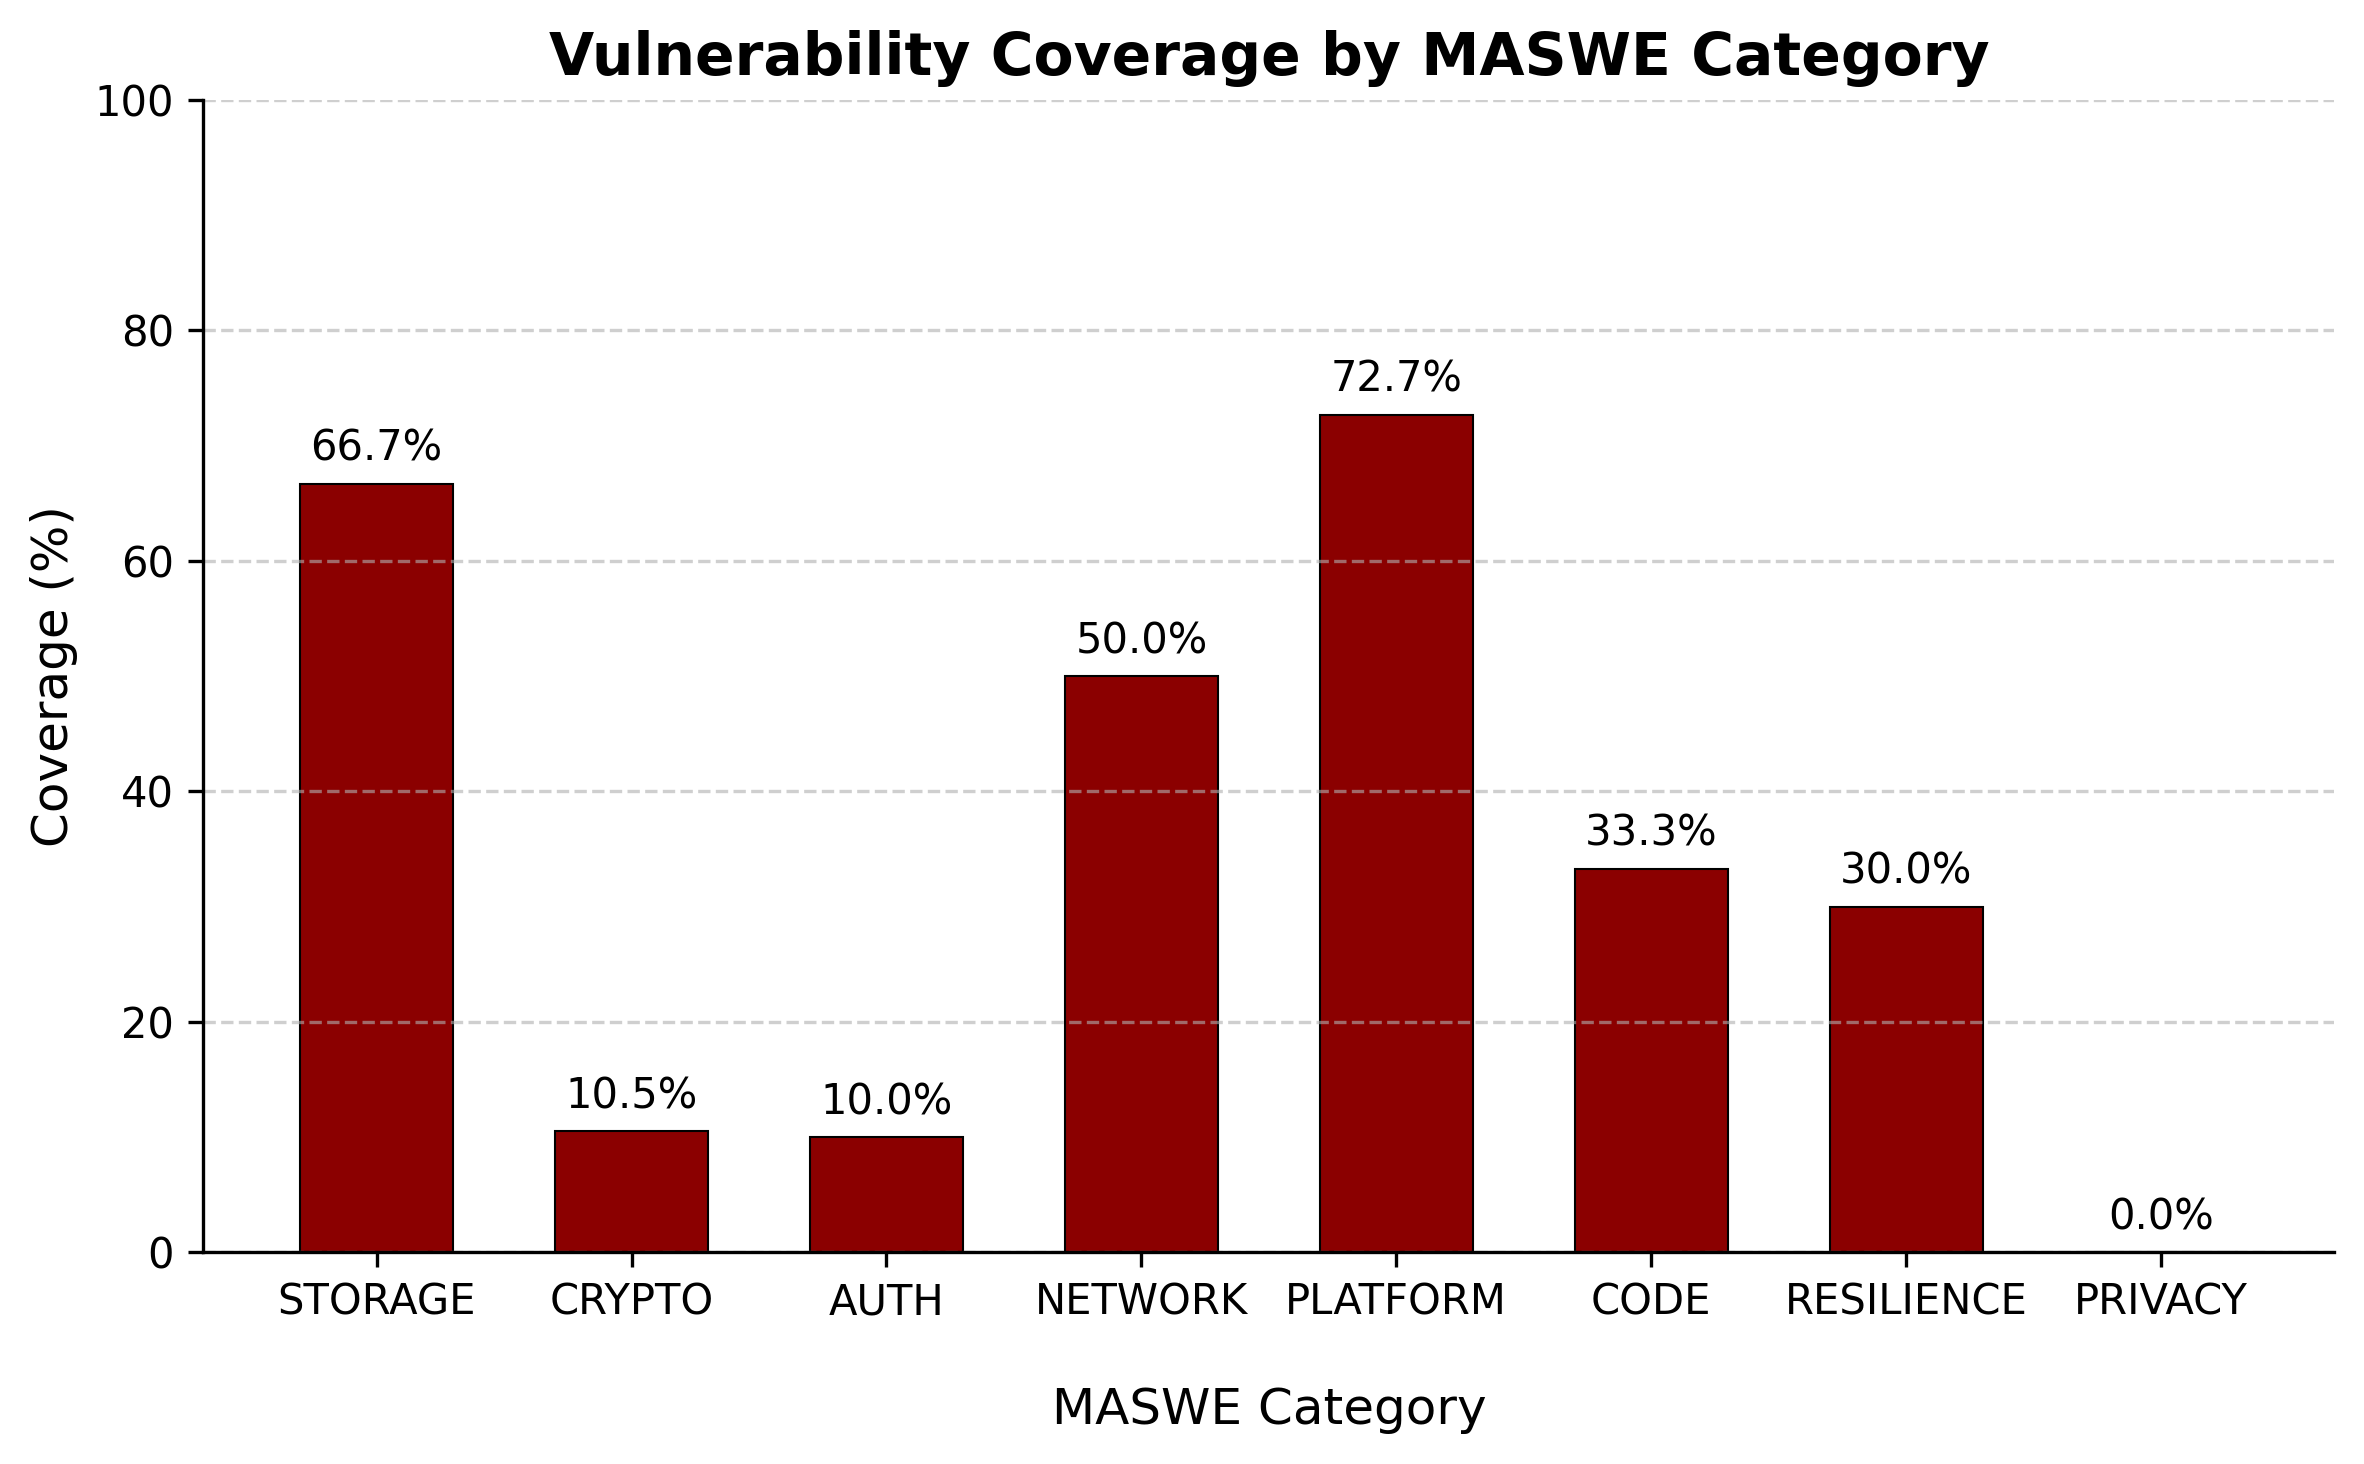
\includegraphics[width=1.0\textwidth]{figures/related_work/vulnerability_coverage_percentage.png}
  \caption{\todo{ADD IMAGE CAPTION}}
  \label{fig:model}
\end{figure}

Viewing the coverage in absolute rather than percentage values makes it look a lot more un-even. As seen in Figure 2.3, all categories have 2 to 6 types of vulnerability types covered, with the only outliers being the category Platform, which has a total of 16 of 22 vulnerabilities implemented, and Privacy, which has no vulnerabilities at all covered. This shows that vulnerabilities are covered rather evenly across the 8 categories, regardless of the amount of vulnerabilities each category has, which explains the large differences in percentage-wise coverage as seen in the previous Figure 2.2. 

The remarkably high coverage of Platform vulnerabilities further enforces the findings of Figure 2.1, meaning that not only are 5 of the 10 most frequently covered vulnerabilities of type Platform, the category itself is also the most broadly implemented category when compared to others. The complete lack of coverage of Privacy vulnerabilities can in part be accounted for by the fact that the category itself is newer than the other 7, only having been introduced in MASVS version 2.1.0. \todo{ADD SOURCE HERE}. Also, the vulnerabilities as described in Privacy are partly more abstract in nature, not necessarily being implementable in the code itself, such as "MASWE-0111: Inadequate Privacy Policy". 

\begin{figure}[htbp]
  \centering
  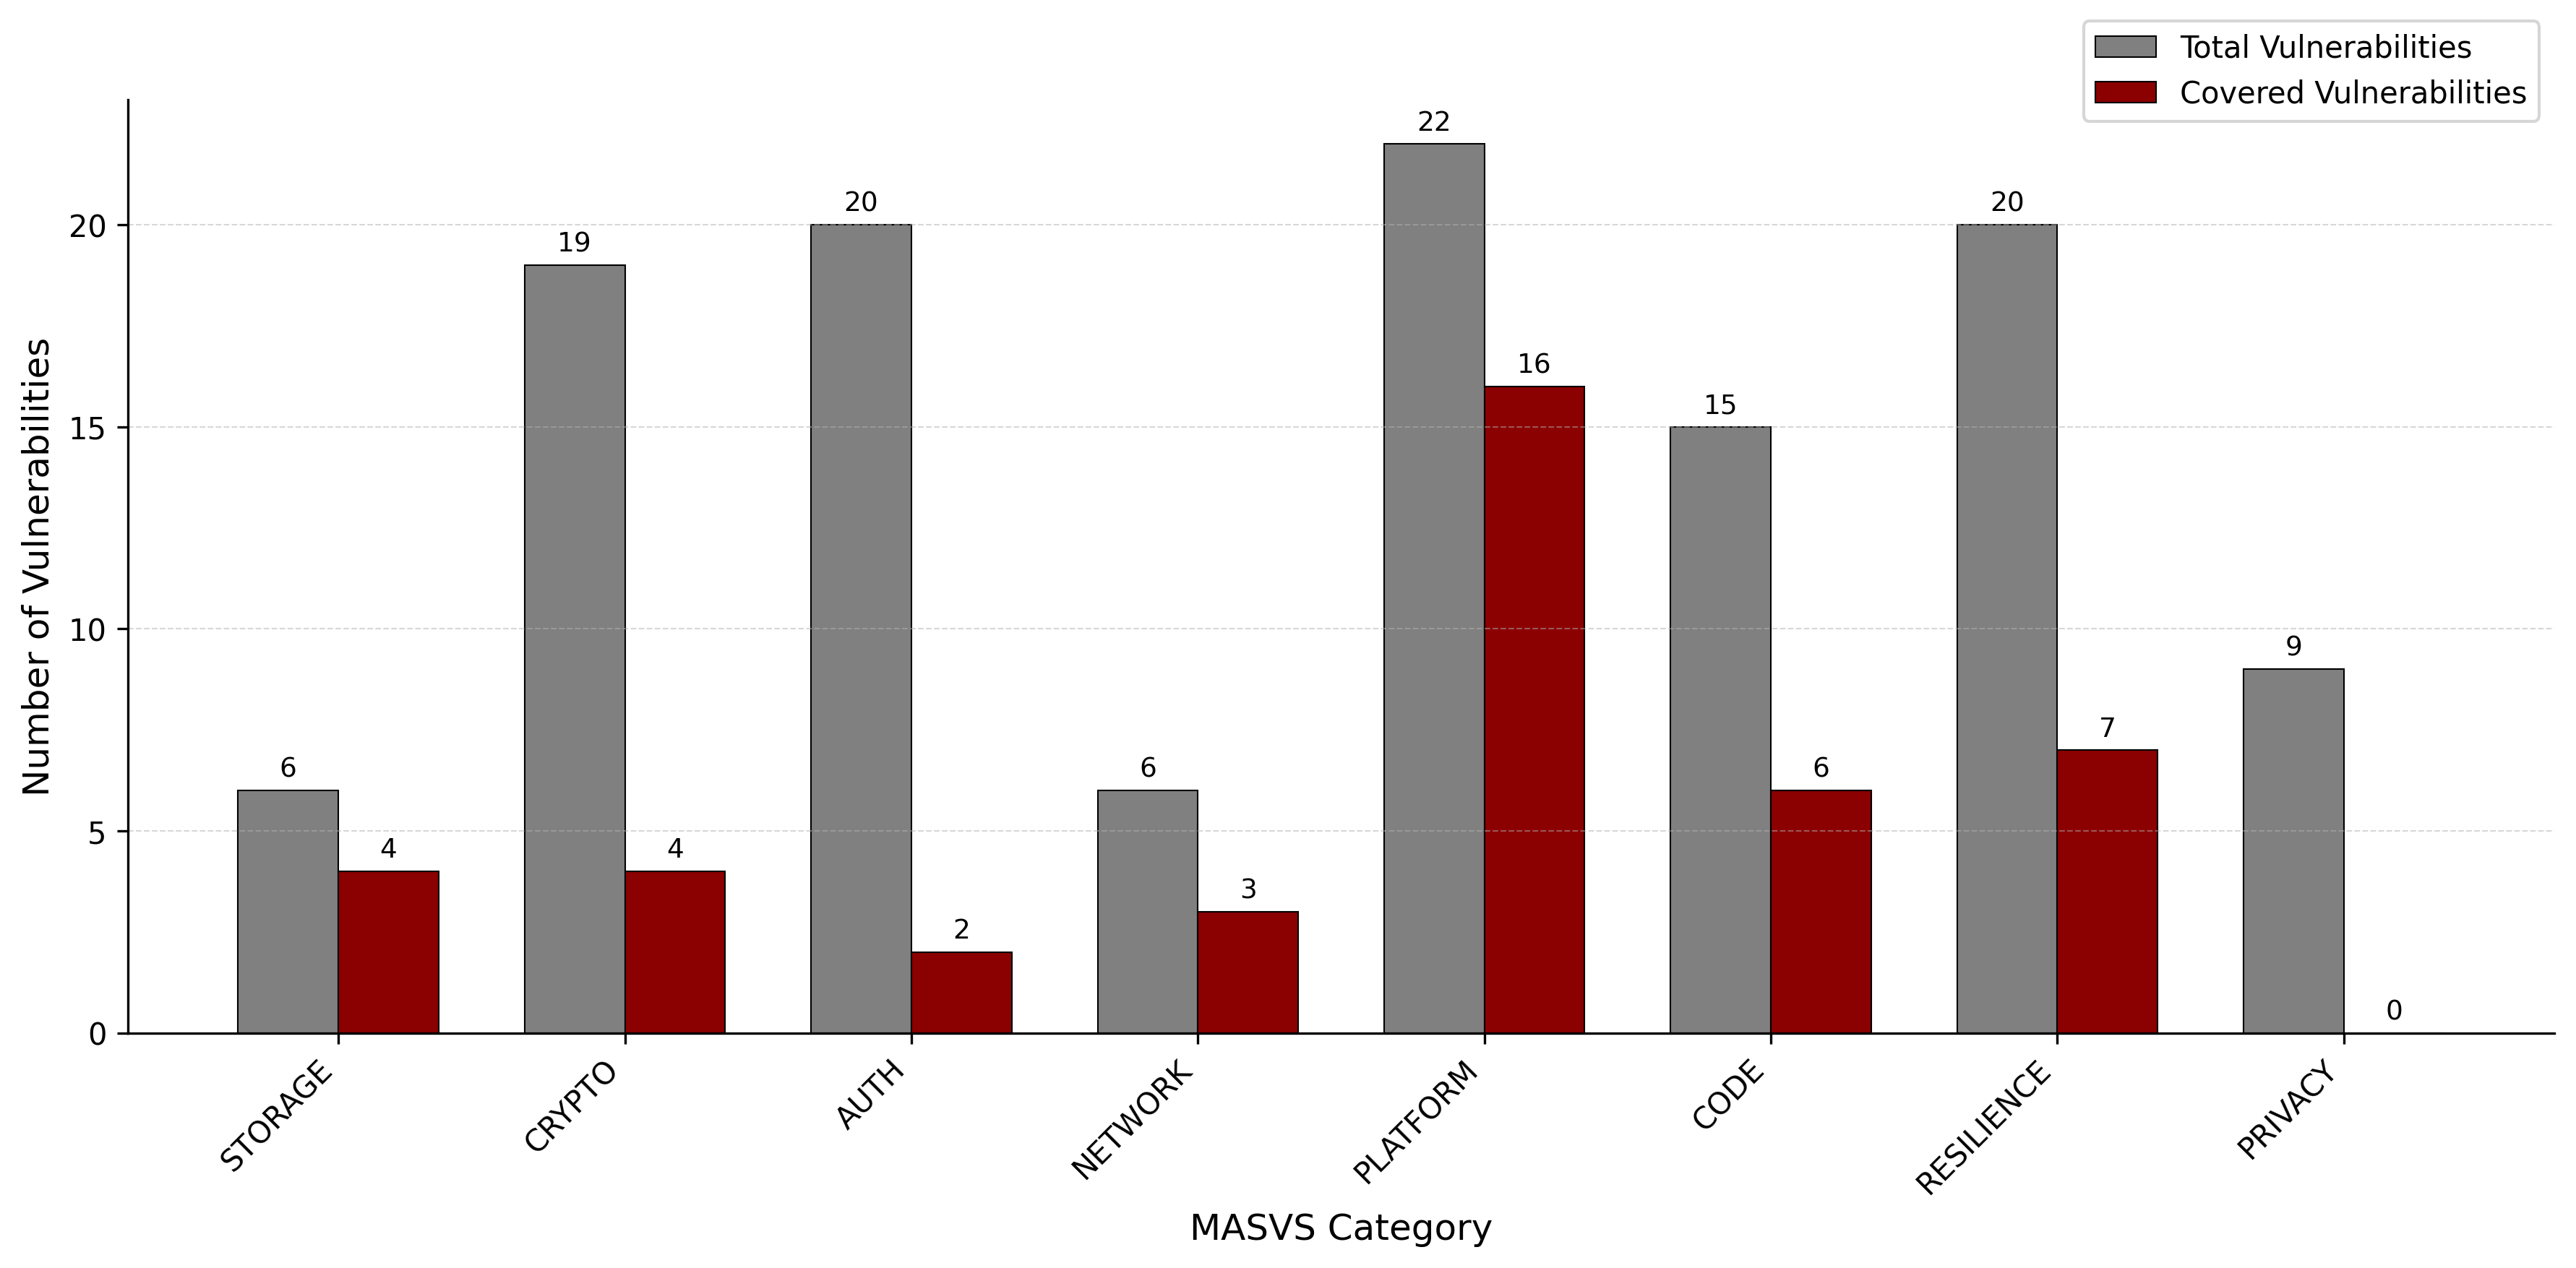
\includegraphics[width=1.0\textwidth]{figures/related_work/vulnerability_coverage_counts.png}
  \caption{\todo{ADD IMAGE CAPTION}}
  \label{fig:model}
\end{figure}

Nevertheless, it can be concluded that the categories are un-evenly covered, with Platform receiving a great deal more of attention than the other categories, and Privacy receiving none. Also, it is clear that the coverage of many categories in these state-of-the-art reference apps is lacking, with only a concerning 10\% of all Crypto and Auth vulnerabilities, as documented by MASWE and tested by MASTG, actually being covered. This despite both of these categories being of great importance, and making up a large part of what mobile security as conducted by OWASP deals with, considering they make up a third (33\%) of all vulnerabilities as documented by MASWE and tested by MASTG.

The reference app developed in this BA thesis aims to solve this issue, by covering the vulnerabilities more broadly, and shifting the focus from over-favoured Categories such as Platform to more neglected ones, such as Crypto and Auth.

% Struktur
\section{Literature Review - Academic relevance of OWASP MASTG}
The OWASP MASTG is the industry standard for mobile app security. But what relevancy does it have in the academic world, and what exactly is it used for? To answer this question, a literature review was conducted, to evaluate papers on their use of the OWASP MASTG, as well as related OWASP parts, e.g. the MASTG reference apps, the MASWE and the MASVS.